\documentclass[11pt]{article}
\usepackage{geometry}
\geometry{
  textheight=8.5in,
  textwidth=6.43in,
  top=1.6cm,
  oddsidemargin=0.24in,
  evensidemargin=0.24in,
  hoffset=-0.5cm
}

\usepackage{graphicx}
\usepackage{xcolor}
\usepackage{listings}
\usepackage{setspace}
\usepackage{array}
\usepackage{amsthm,amsmath,mathtools,amsfonts,amssymb}
\usepackage{url}
\usepackage{booktabs}    % <-- 用 booktabs 美化表格
\usepackage{longtable}
\usepackage{float}
\usepackage{caption}     % <-- caption 先于 subcaption
\usepackage{subcaption}
\usepackage{algorithm}
\usepackage{algpseudocode}
\usepackage{placeins}

% 定理环境定义(必须在导言区)
\newtheorem{theorem}{Theorem}
\newtheorem{lemma}{Lemma}
\newtheorem{proposition}{Proposition}
\newtheorem{definition}{Definition}
\newtheorem{corollary}{Corollary}

% 数学符号定义(使用数学友好的方式)
\DeclarePairedDelimiter{\modd}{|}{|}
\DeclarePairedDelimiter{\norm}{\left|}{\right|}
\DeclarePairedDelimiter{\kh}{(}{)}
\DeclarePairedDelimiter{\zkh}{[}{]}
\DeclarePairedDelimiter{\dkh}{\{}{\}}
\newcommand{\hj}{h_j}
\newcommand{\Mj}{M_j}
\newcommand{\aj}{y_j}
\newcommand{\hjm}{h_{j-1}}

%公式代码颜色定义
\newtagform{mycolour}{\color{cyan}(}{)}
\usetagform{mycolour}

% 文档信息
\title{Interpolation of Gaussian Wave Packet}
\author{Chang.Liu\ $\mathrm{2252377}$}
\date{} % 删除日期

\begin{document}
\maketitle  % 必须在\begin{document}之后

% 重置计数器
\setcounter{page}{1} 
\setcounter{equation}{0}


%Abstract
\begin{abstract}
  
This report employees numerical approximation techniques for a specific function derived from a Gaussian wave 
packet: $f(x) = e^{-x^2/20} \cos(5x)$, over the interval $[-10, 10]$. Accurate representation of such oscillatory functions on 
long domains is crucial in  Physics and Engineering. Initially, I devived Taylor series up to the 30th and 100th 
order around $x=0$. Due to locality, significant error and rapid deterioration of precision away from the expansion point happened, 
particularly when $|x| > 6$. To overcome the limitations of pure Taylor expansion, this study 
explores multi-point interpolation and polynomial fitting methods. Neville's method with equally spaced nodes is implemented, which despite 
showing some improvement over Taylor within limited regions, suffers severely from the Runge phenomenon across the large interval, resulting 
in extreme oscillations and large errors near the boundaries. Subsequently, two alternative strategies are explored: Vandermonde-Arnoldi fitting 
utilizing Chebyshev nodes, and Cubic Spline interpolation. The Vandermonde-Arnoldi method with Chebyshev nodes demonstrates remarkable 
performance, effectively mitigating the Runge phenomenon and achieving exceptionally high accuracy (errors on the order of $10^{-15}$) 
over the entire interval at the order ($n=100$) and higher. Cubic Spline interpolation provides a piecewise smooth approximation; 
its error is observed to correlate with the function's magnitude and decreases with increasing node density, albeit with a slower, approximately 
linear convergence rate and significantly lower overall accuracy compared to the high-order Vandermonde-Arnoldi method. The findings highlight 
the importance of appropriate node selection and the advantages of orthogonal polynomial fitting over standard interpolation for approximating 
complex, oscillatory functions on extended domains.

\end{abstract}

% Introduction
\section{Introduction} 
\subsection{Gaussian Wave Packet}
The Gaussian wave packet was not “discovered” or “invented” by a specific physicist at a particular moment. Its emergence and importance became evident gradually with the 
establishment of quantum mechanical theory itself and the application of mathematical tools such as Fourier analysis. The wave function of a Gaussian wave packet is a Gaussian function (i.e. A bell curve) describing the probability of distribution and solutions to some PDEs. It was firstly put forward by one of the greatest mathematician Gauss.
\begin{equation}
  f(x)=A\mathrm{e}^{-x^2}
\end{equation}
The Gaussian function is a mathematically “well-behaved” function. Particularly, its Fourier transform is also in the from of Gaussian function.
Thus, It was naturally became an ideal choice for constructing such localized wave packets. \\
The Gaussian wave packet also has extensive applications in physics, such as in quantum mechanics, optics, and signal processing.
In quantum mechanics, it can be used to describe the evolution of particles; in optics, it can describe the electric field distribution of laser pulses.$^{[1]}$
In the field of communication, it can also be closely related to the Fourier transform.\\
e.g.(The distribution of the electric field):

\begin{equation}
  E(t) = E_0 \, e^{-\frac{t^2}{2\tau^2}} e^{i\omega_0 t}
\end{equation}

\subsection{This report}
In computational physics and engineering, accurately representing and manipulating such functions numerically is crucial. 
Although the analytical form of a Gaussian wave packet is known, practical scenarios often require its evaluation or processing on 
discrete grids or through approximate representations, especially when dealing with interactions, evolution in complex potentials, 
or integration into larger numerical simulations. This necessitates the application of numerical methods for function approximation.

This project focuses on the numerical approximation of a specific function derived from a Gaussian wave packet.\\
The origional function contains the complex number $\mathrm{i}\in\mathbb{C}$:
\begin{equation}
  f(x) = A \, e^{-a x^2} \, e^{\mathrm{i} k x}
\end{equation}
This formula characterizes the particle's probability distribution in the complex plane; however, in the present analysis, 
we restrict our investigation to the real part of the expression transformed by Euler's formula:\\
\begin{equation}
  f(x) = e^{-\frac{x^2}{20}} \cos(5x), \quad \text{approximation in } [-10, 10]
\end{equation}

This function represents the real part of a particular complex Gaussian wave packet with given parameters. The core aim of my research 
is to explore and compare various numerical techniques for approximating this function within the specified domain. The report will delve 
into different approximation strategies, including methods based on interpolation using various basis functions and fitting techniques, 
applied to both discrete data points derived from the function and potentially continuous representations where applicable. By examining 
these different approaches, this report aims at providing a comparative analysis, evaluating their suitability based on key performance 
indicators such as the accuracy of the approximation achieved, the complexity involved in their implementation, and their computational 
efficiency. The goal is to highlight the advantages and disadvantages of each method in the context of approximating functions with 
Gaussian-like profiles and oscillatory components.


\subsection{Assumption}
In this study, the abbreviation: \\
1."OF" will be strategically deployed as a lexical shorthand for the complete term "original function." \\
2."NM" as "Neville Method".\\
3."VA" as "Vandermonde with Arnoldi Method"
4."CS" as "Cubic Spline Method"
These notational conventions are adopted to achieve syntactic brevity and enhance expository efficiency throughout the analytical framework.

%Numerical Methods
\section{Numerical Methods and Implementation Details} 

\subsection{Taylor series}
Noticed that the interval of the function is symmetric, the two elements of it are also even functions. We shall try pure Taylor expansion
first (Generally, this is also a interpolation with basis $1, x, x^{2}\cdots$at with only one point \{0\}).\\ Below is the Taylor expansion:


\begin{equation}
\setlength{\arraycolsep}{1ex}% 可调列间距
\begin{array}{@{}r@{\;}r@{\;}r@{\;}r@{\;}r@{\;}r@{}}
T_{30}\ =\ 1
&-\displaystyle\frac{251}{20}x^2
&+\displaystyle\frac{62653}{2400}x^4
&-\displaystyle\frac{26735295125}{831849344}x^6
&+\displaystyle\frac{5347059025}{6654794752}x^8
&\\[1ex]
%
& 
&-\displaystyle\frac{26735295125}{3327397376}x^{10}
&+\displaystyle\frac{5347059025}{13309589504}x^{12}
&-\displaystyle\frac{26735295125}{6654794752}x^{14}
&\\[1ex]
%
& 
&+\displaystyle\frac{5347059025}{26619179008}x^{16}
&-\displaystyle\frac{26735295125}{13309589504}x^{18}
&+\displaystyle\frac{5347059025}{53238358016}x^{20}
&\\[1ex]
%
& 
&-\displaystyle\frac{26735295125}{26619179008}x^{22}
&+\displaystyle\frac{5347059025}{106476716032}x^{24}
&-\displaystyle\frac{26735295125}{53238358016}x^{26}
&\\[1ex]
%
& 
&+\displaystyle\frac{5347059025}{212953432064}x^{28}
&-\displaystyle\frac{26735295125}{106476716032}x^{30}
\end{array}
\end{equation}
From the property of Taylor series, higher the power, higher the accuarcy. However, the locality of the Taylor expansion 
fundamentally limits its ability of providing accurate approximations for complex functions when evaluated over a large interval. 
For instance, approximating the function poses a significant challenge for this method. Moreover, the Taylor expansion formula 
for such complex functions tends to be intricate and cumbersome, involving numerous terms with horrible coefficients.\\
Below is the gragh of the origional function and the Taylor series generated from MATLAB:
\begin{figure}[h]
\centering
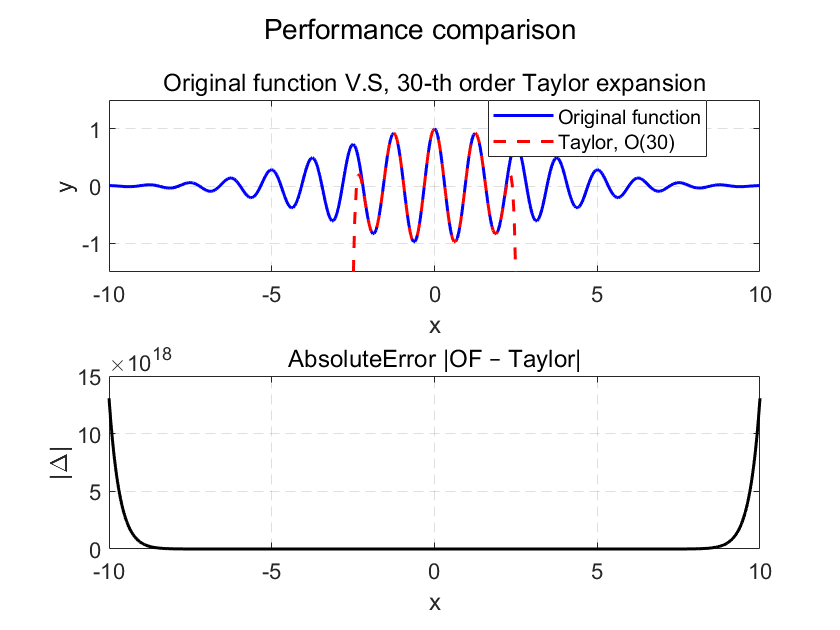
\includegraphics[width=0.51\textwidth]{Taylor.png}
\caption{Taylor expansion}
\end{figure}

The accompanying figure illustrates this limitation by plotting the origional function alongside 
its 30th-order Taylor expansion. The error increases exponentially as $\modd{x}$ gets larger: especially when larger than \{2.2\}. 
Despite extending the expansion to 30th order(this is really a high order), the approximation's 
precision rapidly deteriorates away from the expansion point.\\
\begin{figure}[h]
\centering
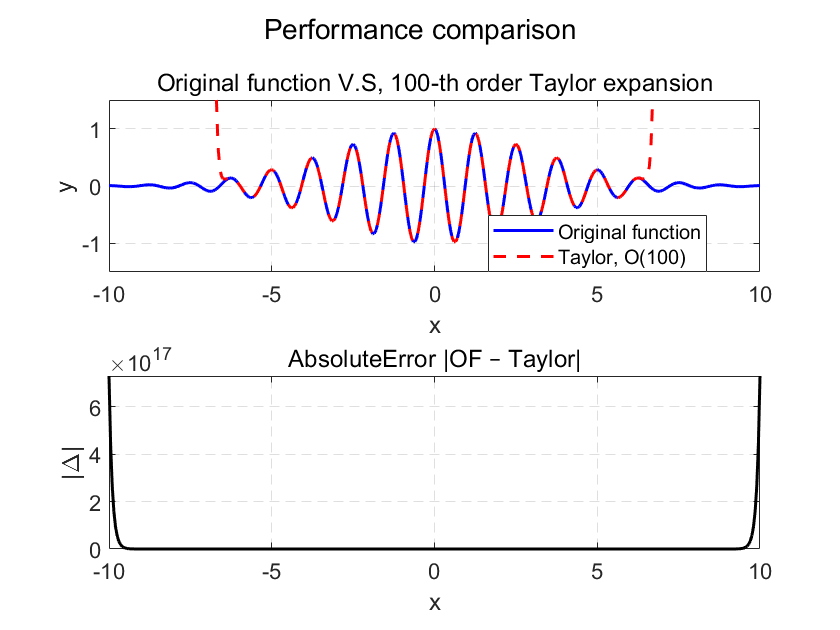
\includegraphics[width=0.7\textwidth]{Taylor2.png}
\caption{Taylor expansion 100-order}
\end{figure}
Even if extended to 100 terms, this series still diverges rapidly around {6}, and its properties are quite poor. Moreover, due to 
the propeerty of the original function,it is quite hard to generate hundreds of derivatives (The number of items will become extremely large, and each item will become very complex). \\
Thus, Taylor formula exhibits significant error in this problem context, 
making it unsuitable for a good global approximation over the interval. Consequently, alternative approximation methods will be explored, 
commencing with an investigation into multi-point interpolation and various polynomial bases.

\subsubsection{Derivatives and Properties}
Before carrying on, I think we should list some orders of derivatives to the function:
\begin{table}[ht]
\centering
\small
\setlength{\tabcolsep}{6pt}   % 列间距
\begin{tabular}{|c|p{0.85\textwidth}|}
\hline
\textbf{Order} & \textbf{expressions}\\
\hline
0 &
\(
 e^{-\frac{x^2}{20}} \cos(5x)
\)\\
\hline
1 &
\(
 -\frac{1}{10}\,e^{-\frac{x^2}{20}}\,x\cos(5x)
 -5\,e^{-\frac{x^2}{20}}\sin(5x)
\)\\
\hline
2 &
\(
 -25\,e^{-\frac{x^2}{20}}\cos(5x)
 +\Bigl(-\frac{1}{10}\,e^{-\frac{x^2}{20}}
       +\frac{1}{100}\,e^{-\frac{x^2}{20}}\,x^2\Bigr)\cos(5x)
 +e^{-\frac{x^2}{20}}\,x\sin(5x)
\)\\
\hline
3 &
\(
 \frac{15}{2}\,e^{-\frac{x^2}{20}}\,x\cos(5x)
 +\Bigl(\frac{3}{100}\,e^{-\frac{x^2}{20}}\,x
        -\frac{1}{1000}\,e^{-\frac{x^2}{20}}\,x^3\Bigr)\cos(5x)
 +125\,e^{-\frac{x^2}{20}}\sin(5x)
 -15\Bigl(-\frac{1}{10}\,e^{-\frac{x^2}{20}}
         +\frac{1}{100}\,e^{-\frac{x^2}{20}}\,x^2\Bigr)\sin(5x)
\)\\
\hline
4 &
\(
 625\,e^{-\frac{x^2}{20}}\cos(5x)
 -150\Bigl(-\frac{1}{10}\,e^{-\frac{x^2}{20}}
          +\frac{1}{100}\,e^{-\frac{x^2}{20}}\,x^2\Bigr)\cos(5x)
 +\Bigl(\frac{3}{100}\,e^{-\frac{x^2}{20}}
         -\frac{3}{500}\,e^{-\frac{x^2}{20}}\,x^2
         +\frac{1}{10000}\,e^{-\frac{x^2}{20}}\,x^4\Bigr)\cos(5x)
 -50\,e^{-\frac{x^2}{20}}\,x\sin(5x)
 -20\Bigl(\frac{3}{100}\,e^{-\frac{x^2}{20}}\,x
         -\frac{1}{1000}\,e^{-\frac{x^2}{20}}\,x^3\Bigr)\sin(5x)
\)\\
\hline
\end{tabular}
\caption{4 orders of derivative}
\end{table} 

Furthermore, the complexity of this function can be attributed to two key characteristics:\\
Firstly, the function exhibits rapid oscillations within the interval. \\
Secondly, the amplitude of these oscillations diminishes progressively near the domain boundaries, resulting in smoother 
variations as the function approaches the edges. \\
Such features necessitate careful analytical treatment, particularly when evaluating convergence properties 
and error analysis.


\subsection{Neville's Method with Equal Spaced Nodes}
Before delving into the detailed process, we will first use a simple and basic method to explore the situation and conduct targeted analysis of the problems that arise.
\subsubsection{The principle of the method}
First, we shall take the nodes. Due to the extreme value highly relates to the $Cos(5x)$ term(a periodic function), we can derive the nodes as 
equal spaced nodes. Although the extreme value also corresponds to $e^{-\frac{x^{2}}{20}}$ and small shifts of apexes does makes differences, 
inqualed nodes will make it inefficient constructing interpolation polynomials.
The polynomial crossing the nodes near the extreme values should have better properties. Due to the choosen of inner nodes, the boundray will not 
be considered(This is a open interpolation due to the largest node is very close to the boundareis).\\
The table displays all the nodes lies in the interval:\\ 


\small
\begin{longtable}{|r|c|r|}
  \caption{Value of $f(x)$ at $x=k\pi/5\;(k=-15,\dots,15)$}\label{tab:fx}\\
  \hline
  \textbf{$k$} & \textbf{$x=k\pi/5$} & \textbf{$f(x)$} \\ \hline\hline
  -15 & $-3\pi$             & -0.0117804 \\ \hline
  -14 & $-\tfrac{14\pi}{5}$ &  0.0208816 \\ \hline
  -13 & $-\tfrac{13\pi}{5}$ & -0.0355816 \\ \hline
  -12 & $-\tfrac{12\pi}{5}$ &  0.0582829 \\ \hline
  -11 & $-\tfrac{11\pi}{5}$ & -0.0917723 \\ \hline
  -10 & $-2\pi$             &  0.1389110 \\ \hline
   -9 & $-\tfrac{9\pi}{5}$  & -0.2021240 \\ \hline
   -8 & $-\tfrac{8\pi}{5}$  &  0.2827170 \\ \hline
   -7 & $-\tfrac{7\pi}{5}$  & -0.3801380 \\ \hline
   -6 & $-\tfrac{6\pi}{5}$  &  0.4913440 \\ \hline
   -5 & $-\pi$              & -0.6104980 \\ \hline
   -4 & $-\tfrac{4\pi}{5}$  &  0.7291850 \\ \hline
   -3 & $-\tfrac{3\pi}{5}$  & -0.8372330 \\ \hline
   -2 & $-\tfrac{2\pi}{5}$  &  0.9240800 \\ \hline
   -1 & $-\tfrac{\pi}{5}$   & -0.9804540 \\ \hline
    0 & $0$                 &  1.0000000 \\ \hline
    1 & $\tfrac{\pi}{5}$    & -0.9804540 \\ \hline
    2 & $\tfrac{2\pi}{5}$   &  0.9240800 \\ \hline
    3 & $\tfrac{3\pi}{5}$   & -0.8372330 \\ \hline
    4 & $\tfrac{4\pi}{5}$   &  0.7291850 \\ \hline
    5 & $\pi$               & -0.6104980 \\ \hline
    6 & $\tfrac{6\pi}{5}$   &  0.4913440 \\ \hline
    7 & $\tfrac{7\pi}{5}$   & -0.3801380 \\ \hline
    8 & $\tfrac{8\pi}{5}$   &  0.2827170 \\ \hline
    9 & $\tfrac{9\pi}{5}$   & -0.2021240 \\ \hline
   10 & $2\pi$              &  0.1389110 \\ \hline
   11 & $\tfrac{11\pi}{5}$  & -0.0917723 \\ \hline
   12 & $\tfrac{12\pi}{5}$  &  0.0582829 \\ \hline
   13 & $\tfrac{13\pi}{5}$  & -0.0355816 \\ \hline
   14 & $\tfrac{14\pi}{5}$  &  0.0208816 \\ \hline
   15 & $3\pi$             & -0.0117804 \\ \hline
\end{longtable}

From the lecture slides, we have known that for any interpolation methods, we will always get the same result if the nodes and
the order of polynomials reduced are the same. Thus, I chose one of the fastest methods of generating polynomials: Neville's method.
The formula of Neville's method are listed below:


\begin{equation}\label{eq:neville-triangle}
\begin{array}{c|cccccc}
   & j=0     & j=1         & j=2           & j=3           & \cdots & j=n      \\ \hline
i=0 & P_{0,0}=f(x_0)
       & P_{0,1}(x)
                    & P_{0,2}(x)
                                  & P_{0,3}(x)
                                                & \cdots & P_{0,n}(x) \\[1ex]
i=1 & P_{1,0}=f(x_1)
       & P_{1,1}(x)
                    & P_{1,2}(x)
                                  & P_{1,3}(x)
                                                & \cdots &          \\[1ex]
i=2 & P_{2,0}=f(x_2)
       & P_{2,1}(x)
                    & P_{2,2}(x)
                                  & \cdots      &        &          \\[1ex]
\vdots
    & \vdots   & \vdots      &             &            & \ddots & \vdots   \\[1ex]
i=n & P_{n,0}=f(x_n)
       &            &             &            &        &          
\end{array}
\end{equation}

Where:  
\begin{align}
P_{i,0}(x) &= f(x_i), 
   \quad i=0,1,\dots,n, \\[6pt]
P_{i,1}(x)
  &= \frac{(x - x_i)\,f(x_{i+1})
         - (x - x_{i+1})\,f(x_i)}{x_{i+1}-x_i},
   \quad i=0,1,\dots,n-1, \\[6pt]
P_{i,2}(x)
  &= \frac{(x - x_i)\,P_{i+1,1}(x)
         - (x - x_{i+2})\,P_{i,1}(x)}
        {x_{i+2}-x_i},
   \quad i=0,1,\dots,n-2, \\[6pt]
&\;\;\vdots \notag\\
P_{i,j}(x)
  &= \frac{(x - x_i)\,P_{i+1,j-1}(x)
         - (x - x_{i+j})\,P_{i,j-1}(x)}
        {x_{i+j}-x_i},
   \ j=1,2,\dots,n,\;i=0,1,\dots,n-j.
\end{align}

Finally, the interpolation polynomial is:
\begin{equation}
P(x)\;=\;P_{0,n}(x)\,.
\end{equation}


\subsubsection{Visualization and Error of NM}
The curves of functions are displayed below, followed by the absolute error. From the graph of the polynomial, we found that the
$P_n(x)$, can approximate $f(x)$ in the interval, much better than taylor expansion. However, x approaching ${9}$, the polynomial oscillating 
extremely: quickly reached the order of magnitudes of $10^{6}$. That is: runge phenomena happened, the filling function moves(jumps) rapidly near 
the boundary.
% 在两张旧图之前加一个 FloatBarrier(可选),防止之前的浮动体往后飘
\FloatBarrier

\begin{figure}[H]
  \centering
  \begin{subfigure}[t]{0.48\textwidth}
    \centering
    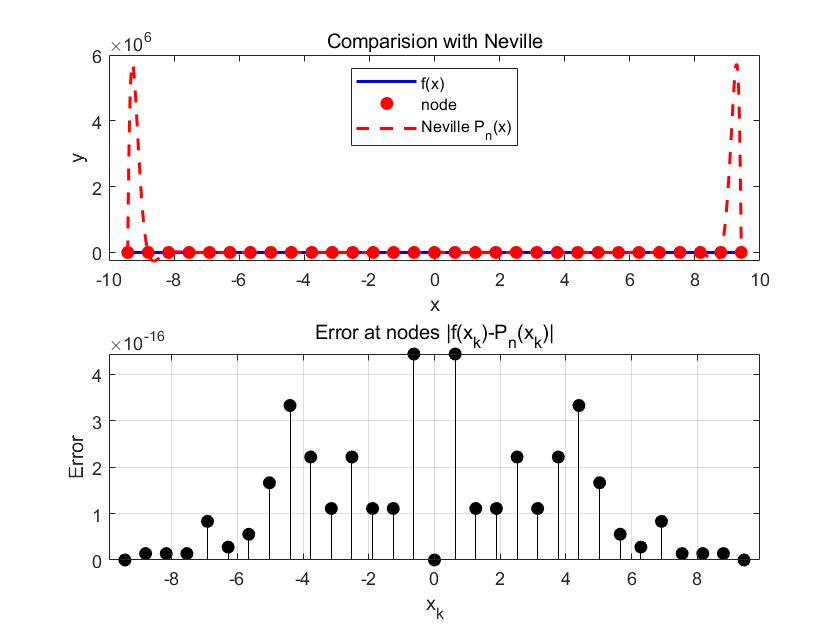
\includegraphics[width=\textwidth]{Neville.png}
    \caption{Neville Interpolation (whole domain)}
    \label{fig:nev_whole}
  \end{subfigure}
  \hfill
  \begin{subfigure}[t]{0.48\textwidth}
    \centering
    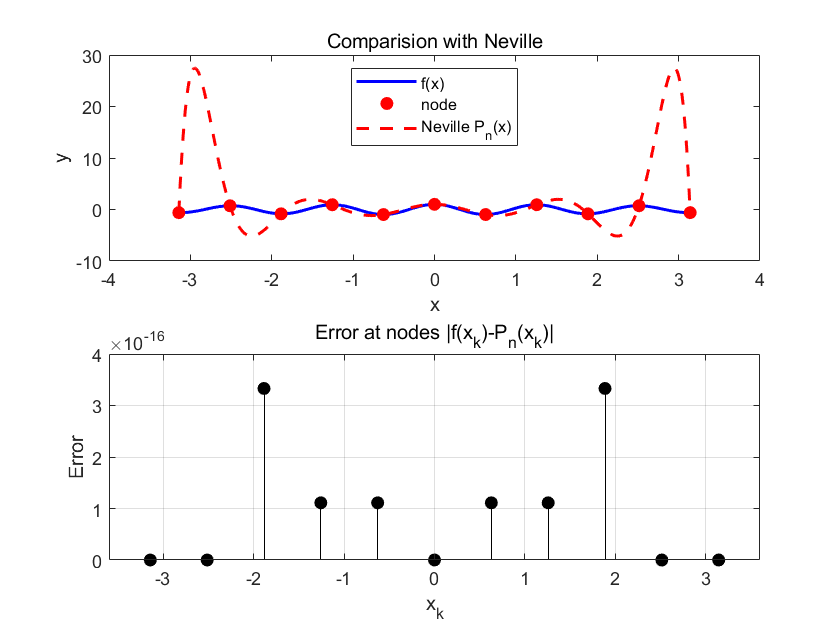
\includegraphics[width=\textwidth]{Neville1.png}
    \caption{Neville Interpolation (smaller domain)}
    \label{fig:nev_small}
  \end{subfigure}
  \caption{Comparison of Neville interpolation on the full interval and a zoomed-in region}
  \label{fig:nev_compare}
\end{figure}

\FloatBarrier

From the picutres, we can clearly found that the high order polynomial has Runge phynomina when $\modd{x}>1.3$. Moreover, its performance is only marginally 
better than that of Taylor. Therefore, we will not delve into a detailed analysis of the errors here.


\subsubsection{Section Review and Analysis}
The Runge phenomenon can be readily identified as arising from two principal causes. The first is the selection of equidistant interpolation 
nodes, a distribution that significantly amplifies errors and induces severe oscillations in the interpolating polynomial, especially towards 
the interval's endpoints. The underlying mechanism for this behavior is as follows:\\

\begin{equation}
\label{eq:interpolation_error} 
f(x) - p_n(x) = \frac{f^{(n+1)}(\xi(x))}{(n+1)!} \prod_{i=0}^{n} (x - x_i)
\end{equation}


\begin{equation}
\label{eq:interpolation_error_norm} % 可选:添加一个标签方便引用
\norm{f(x) - p_n(x)} = \mathrm{max}\norm{\frac{f^{(n+1)}(\xi(x))}{(n+1)!}}\times\  \mathrm{max}\norm{\prod_{i=0}^{n} (x - x_i)}
\end{equation}

We should do something to make the second term smaller because the value of derivatives are bounded by the function itself\\
The second factor is the limitation 
of standard polynomial interpolation to solely match function values at the interpolation points, thereby neglecting crucial information 
regarding the function's derivatives or other intrinsic properties. Accordingly, the focus of the following sections will be directed towards 
methodologies designed to mitigate the issues associated with these two characteristics.\\


\subsection{Vandermonde with Arnoldi alongwith Chebyshev nodes}
\subsubsection{Thought Flow}
We attempt changing the nodes in the beginning.\\
First of all, to eliminate the error caused by the multiplication of polynomial nodes, we can use Chebyshev nodes. Furthermore, we do not need 
to strictly make the polynomial pass exactly through every interpolation point. \\
Furthermore, we can approximate the original function using polynomial 
approximation in the same way as linear regression. This method has evolved into using the Vandermonde-Arnoldi matrix$^{[2]}$ at 
Chebyshev nodes. In this way, it can simultaneously solve the two problems encountered in the previous method.

\subsubsection{Mathematical Details}
Chebyshev Nodes:\\
Chebyshev nodes are defined by Chebyshev polynomials. 
The nodes generated by this method will be densely distributed near the boundaries, restricting the polynomial's 
ability to move around near the boundaries: hereby reducing the undesirable oscillations produced by the polynomial 
near the boundaries.\\
The following three formulas respectively represent: Chebyshev polynomials, unit nodes, and nodes mapped onto any interval:

  \begin{equation}
    T_{n}(x)=\cos\!\bigl(n\arccos x\bigr),\quad n=0,1,2,\dots,\;x\in[-1,1].
  \end{equation}
  \begin{equation}
    x_k^{*}
    =\cos\!\Bigl(\frac{(2k+1)\pi}{2(n+1)}\Bigr),\quad k=0,1,\dots,n.
  \end{equation}
  \begin{equation}
    x_k
    =\frac{a+b}{2}
     +\frac{b-a}{2}\,
      \cos\!\Bigl(\frac{(2k+1)\pi}{2(n+1)}\Bigr),
    \quad k=0,1,\dots,n.
  \end{equation}



Vandermonde-Arnoldi:\\
\begin{algorithm}[H]
\caption{Arnoldi--Vandermonde polynomial fitting}\label{alg:arnoldiVand}
\begin{algorithmic}[1]
  \Require $f:[a,b]\to\mathbb R$, order $n$.
  \State $m\gets n+1$.
  \State Construct Chebyshev nodes:
    \[
      x_k=\tfrac{a+b}{2}+\tfrac{b-a}{2}\cos\!\bigl(\tfrac{\pi k}{n}\bigr),
      \;k=0,\dots,n.
    \]
  \State $f_k\gets f(x_k)$,\,$k=0,\dots,n$.
  \State $Q(:,1)\gets \mathbf1,\;H\gets0\in\mathbb R^{m\times n}$.
  \For{$k=1:n$}
    \State $v\gets x\.*Q(:,k)$
    \For{$j=0:k-1$}
      \State $H(j+1,k)\gets\frac1m\,Q(:,j+1)^T v$
      \State $v\gets v - H(j+1,k)\,Q(:,j+1)$
    \EndFor
    \State $H(k+1,k)\gets\|v\|_2/\sqrt{m},\;
           Q(:,k+1)\gets v/H(k+1,k)$
  \EndFor
  \State $d\gets \frac1m\,Q^T\,(f_0,\dots,f_n)^T$.
  \Ensure $p_n(x)=\sum_{k=0}^n d_k q_k(x)$.
\end{algorithmic}
\end{algorithm}


\subsubsection{Visualization and Error of VA}


\FloatBarrier
\begin{figure}[H]
  \centering
  \begin{subfigure}[t]{0.484\textwidth}
    \centering
    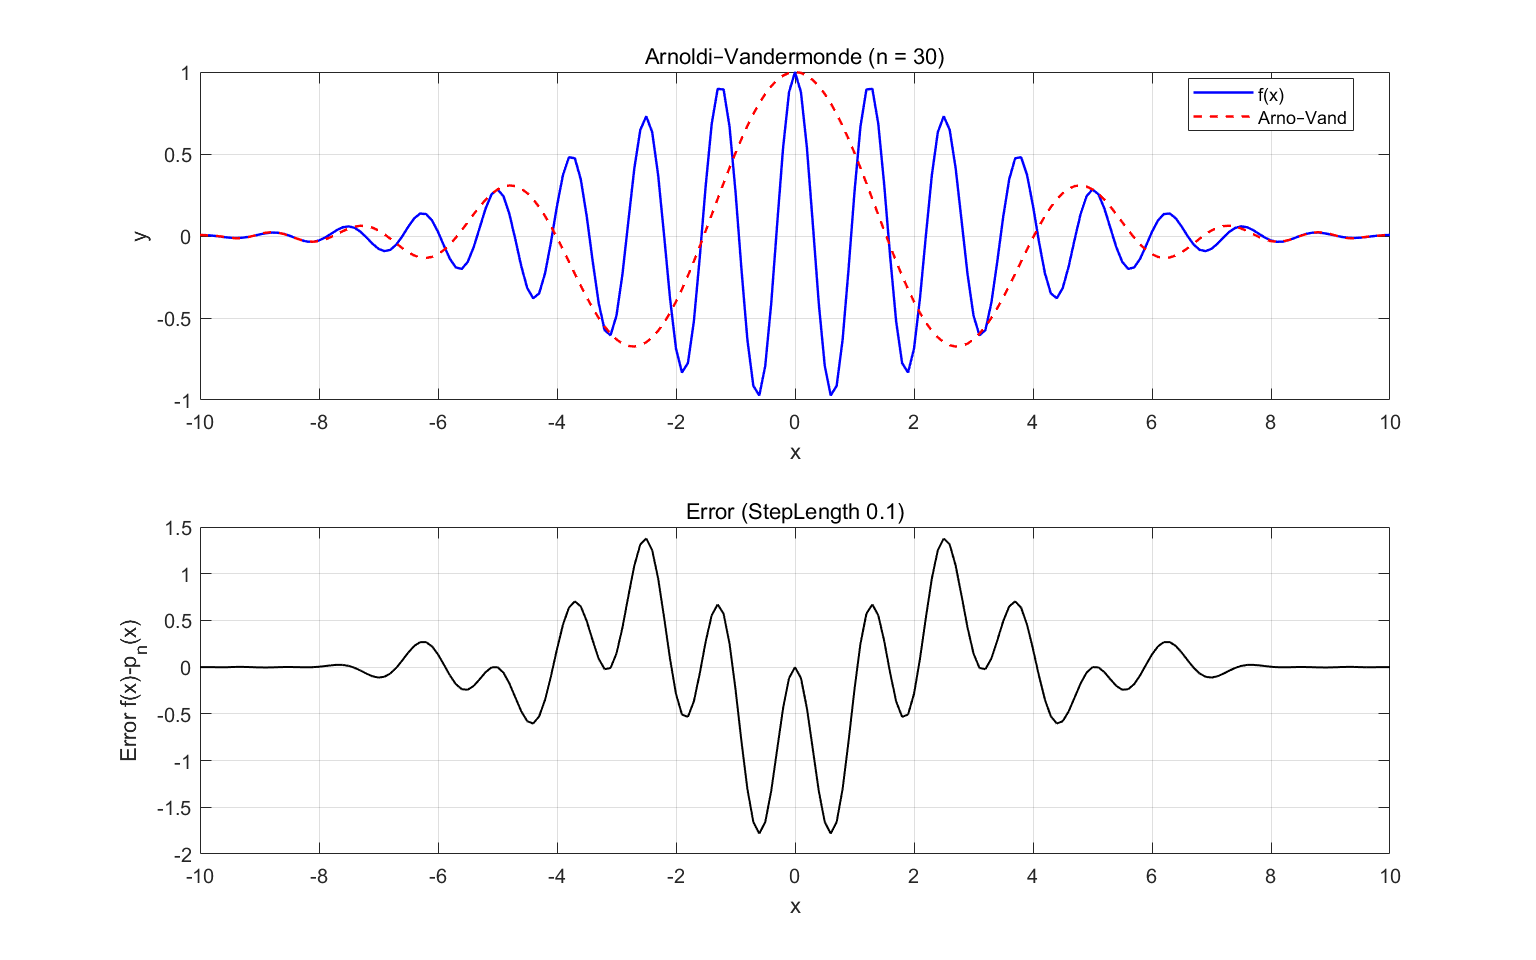
\includegraphics[width=\textwidth]{VA30.png}
    \caption{Vandermonde-Arnoldi (n=30)}
    \label{fig:nev_whole1}
  \end{subfigure}
  \hfill
  \begin{subfigure}[t]{0.48\textwidth}
    \centering
    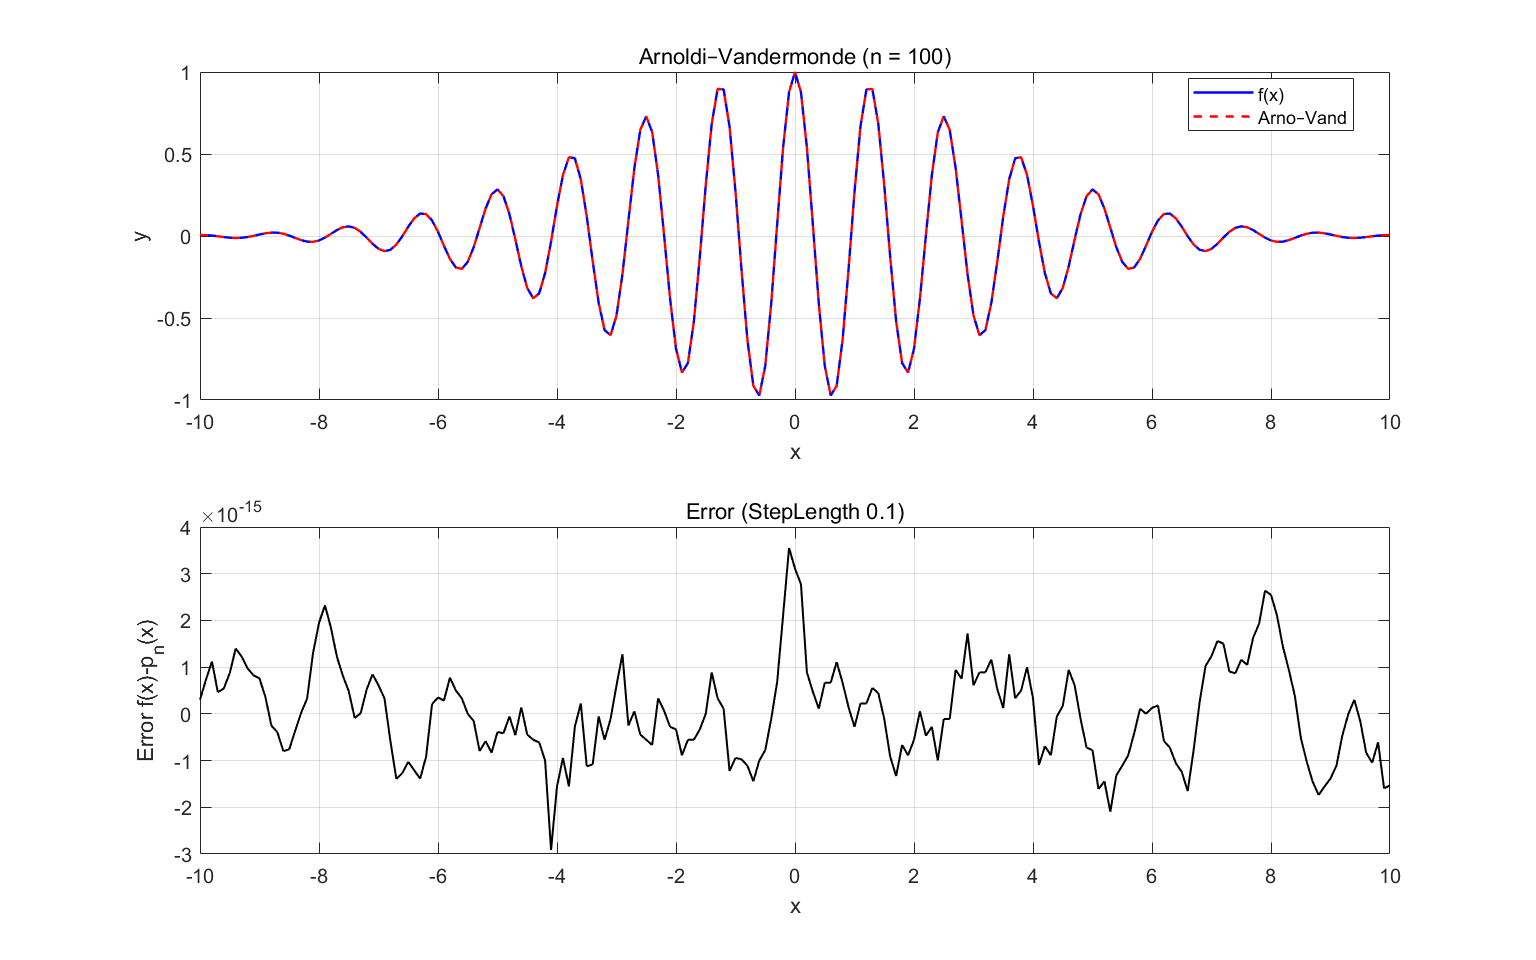
\includegraphics[width=\textwidth]{VA100.png}
    \caption{Vandermonde-Arnoldi (n=100)}
    \label{fig:nev_small1}
  \end{subfigure}
  \caption{Vandermonde-Arnoldi with different orders}
  \label{fig:nev_compare1}
  \begin{subfigure}[t]{0.58\textwidth}
    \centering
    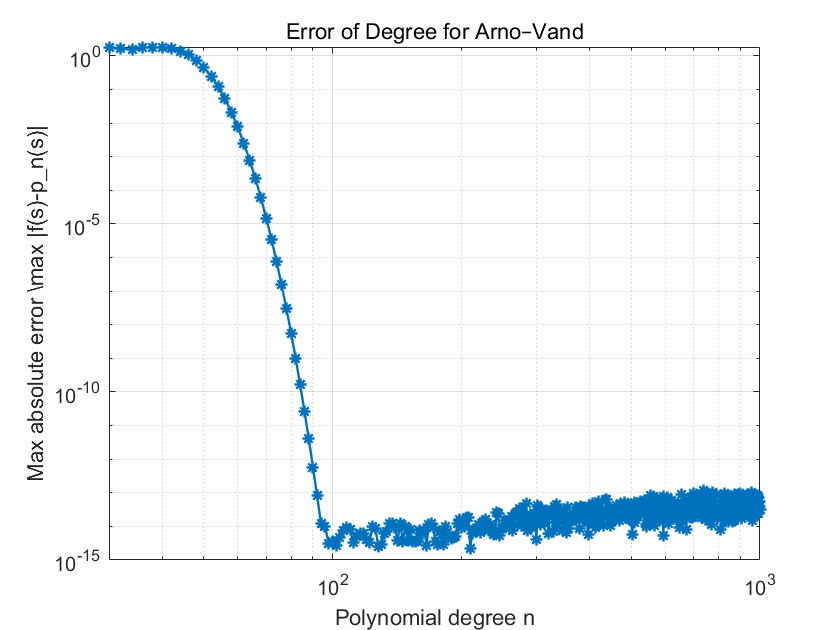
\includegraphics[width=\textwidth]{ErrorVA.png}
    \caption{Error with log-log axis}
    \label{fig:nev_small1}
  \end{subfigure}
  \caption{Vandermonde-Arnoldi with different orders}
  \label{fig:nev_compare11}
\end{figure}
    
  
\FloatBarrier

By examining the upper two images, we found that the result of the VA fitting was not very accurate at the 30th order, 
but it performed extremely well at the 100th order, with the error even at the $10^{-15}$ order of magnitude(Same result with the referenced article).\\
This function not only does not exhibit the Runge phenomenon at the 100th order, but also runs very effectively. 
Under the condition of error detection with a step size of 0.1, almost all the points closely follow the original function. 
It is not difficult to observe that the high-order VA method is very effective when fitting long intervals and functions with 
multiple oscillations. \\
What's more interesting is that: while we increase the polynomial degree to achieve higher accuracy, the Chebyshev nodes also 
increase the number of nodes: in turn, limits the Runge phenomenon of high-order polynomials. VA with Chebyshev nodes has a great property: self-stability.
However, $10^{-15}$ seems to be the precision limit of this method. I ranged n from 30 to 1000. We can see the algorithm has reached the limit when n = 100. From then on, 
the precision can only fluctuate around a certain value (around $10^{-14}$). Due to the reasons of approximate orthogonalization and computer 
rounding errors, the precision and error will cancel each other out, and eventually approach a stable value.$^{[3]}$

\subsection{Cubic Spline}
\subsubsection{Thought Flow}
The VA method addresses the Runge phenomenon (essentially the error in fitting) in terms of node selection efficiently. 
Now, we are attempting to solve the error problem using a method that conducts a deep analysis of the curve's properties. \\
Currently, there is a method that employs low-degree polynomials, functions, and their derivatives for fitting: spline interpolation. 
To better fit this curve, we use cubic spline interpolation.

\subsubsection{Mathematical Details}
The reason for using cubic splines here is as follows: \\
1. It can fit the original function using higher-order derivatives. \\
2. It uses independent cubic functions between the nodes instead of a single complete function. \\
These are the two reasons why I consider cubic spline interpolation to be better than Hermite interpolation (which is not used in this article).\\
The definition and condition of CS are list below:
% 定义 M_j
\[
  M_j := S''(x_j),\quad j=0,1,\dots,n.
\]

% 分段三次样条的构造条件
\begin{subequations}\label{eq:spline-conds}
\begin{align}
  &\text{(a) }S_j(x)\text{ is a cubic polynomial on }[x_j,x_{j+1}],\quad j=0,1,\dots,n-1;\\
  &\text{(b) }S_j(x_j)=f(x_j),\quad S_j(x_{j+1})=f(x_{j+1}),\quad j=0,1,\dots,n-1;\\
  &\text{(c) }S_j(x_{j+1})=S_{j+1}(x_{j+1}),\quad j=0,1,\dots,n-2;\\
  &\text{(d) }S_j'(x_{j+1})=S_{j+1}'(x_{j+1}),\quad j=0,1,\dots,n-2;\\
  &\text{(e) }S_j''(x_{j+1})=S_{j+1}''(x_{j+1}),\quad j=0,1,\dots,n-2.
\end{align}
\end{subequations}

% 边界条件(任选其一)
\paragraph{Natural Boundry(Free):}
\[
  M(x_0)=0,\quad M(x_n)=0.
\]


% --- 公式1:分段三次样条表达式 ---
\begin{equation}\label{eq:cubic-spline-piece}
S_j(x)\;=\;
\frac{(x_{j+1}-x)^3\,M_j + (x - x_j)^3\,M_{j+1}}{6\,h_j}
\;+\;
\biggl(\frac{y_j}{h_j}-\frac{h_j\,M_j}{6}\biggr)(x_{j+1}-x)
\;+\;
\biggl(\frac{y_{j+1}}{h_j}-\frac{h_j\,M_{j+1}}{6}\biggr)(x - x_j),
\end{equation}
Where:
\[
h_j = x_{j+1}-x_j,\quad
M_j = S''(x_j),\quad
y_j = f(x_j).
\]

% --- 公式2:自然边界条件下的 M_j 三对角线性方程组 ---
\begin{equation}\label{eq:cubic-spline-tridiag}
\hjm\,M_{j-1}
\;+\;2\bigl(\hjm+\hj\bigr)\,M_j
\;+\;\hj\,M_{j+1}
\;=\;
6\;\Bigl(\frac{y_{j+1}-y_j}{\hj}-\frac{y_j-y_{j-1}}{\hjm}\Bigr),
\quad j=1,2,\dots,n-1,
\end{equation}
Combined with natural boundaries: 
\[
M_0=0,\quad M_n=0.
\]
Solve all: \(M_j\), plug them into quation $(18)$ obtain the final piecewise interpolation function.

\subsubsection{Visualization and Error of CS}

Firstly, we only use the equally spaced nodes mentioned above for interpolation:
\FloatBarrier

\begin{figure}[H]
  \centering
  \begin{subfigure}[t]{0.48\textwidth}
    \centering
    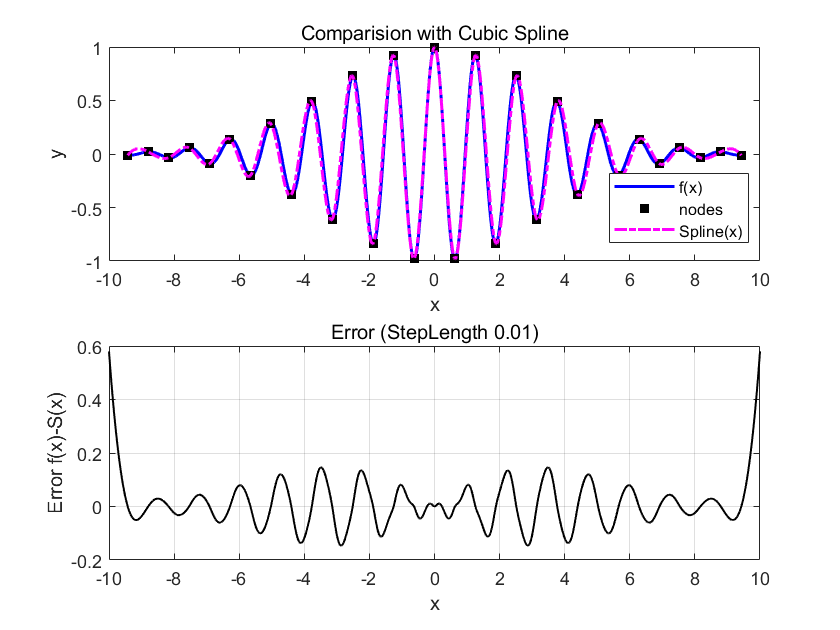
\includegraphics[width=\textwidth]{CubicSpline.png}
    \caption{Cubic-Spline (whole domain)}
    \label{fig:nev_whole0}
  \end{subfigure}
  \hfill
  \begin{subfigure}[t]{0.48\textwidth}
    \centering
    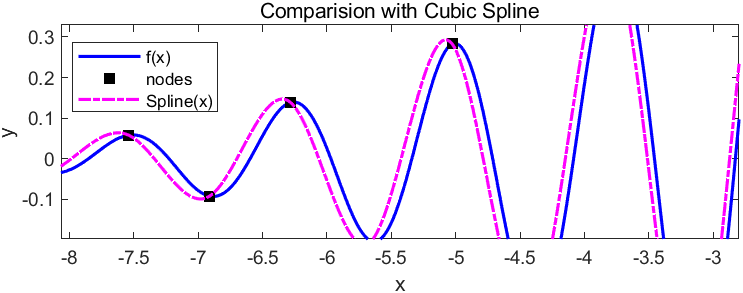
\includegraphics[width=\textwidth]{Spline2.png}
    \caption{Cubic-Spline (zoomed domain)}
    \label{fig:nev_small0}
  \end{subfigure}
  \caption{Comparison of Cubic Spline on the full interval and a zoomed-in region}
  \label{fig:nev_compare0}
\end{figure}

\FloatBarrier
From the zoomed graph, the fitting function will have a slight stretch near the boundary: 
the shapes are similar, but the abscissa is approximately multiplied by a constant.\\

Then, we added the boundary points and the zeros of the function. This operation is reasonable: place the nodes at the key positions of the function's fluctuations-the 
zero points (defining the period/phase) and the extreme points (defining the amplitude). Thus, each spline segment typically covers only 
a part of the waveform (from the zero point to the peak, from the peak to the zero point, from the zero point to the trough, from 
the trough to the zero point), which can most effectively capture the shape and oscillation characteristics of the function and provide 
a better fitting curve. The result is listed below: 
\FloatBarrier
\begin{figure}[H]           % ← 注意这里是方括号
  \centering
  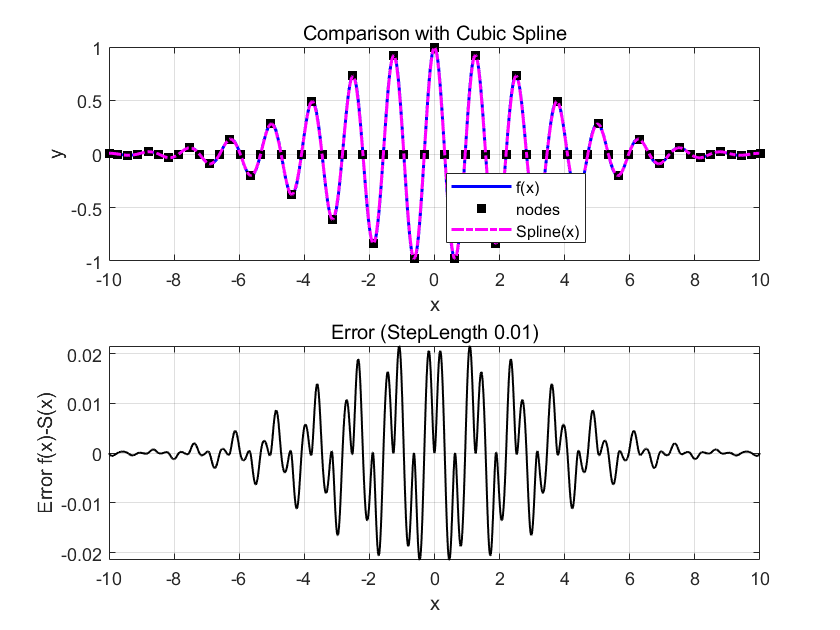
\includegraphics[width=0.6\textwidth]{CS2.png}
  \caption{Cubic-Spline (added boundary and zero points)}
  \label{fig:nev_added}
\end{figure}
\FloatBarrier
We can draw such a conclusion: the value of the error is also constantly oscillating: at the nodes, 
the zeros are taken, and in the range between the nodes, it increases. Therefore, we hope to reduce the "intermediate error" 
by continuously increasing the number of nodes between the nodes.\\
Final version: added two and four points between each node based on the original configuration:

\FloatBarrier
\begin{figure}[H]
  \centering
  \begin{subfigure}[t]{0.48\textwidth}
    \centering
    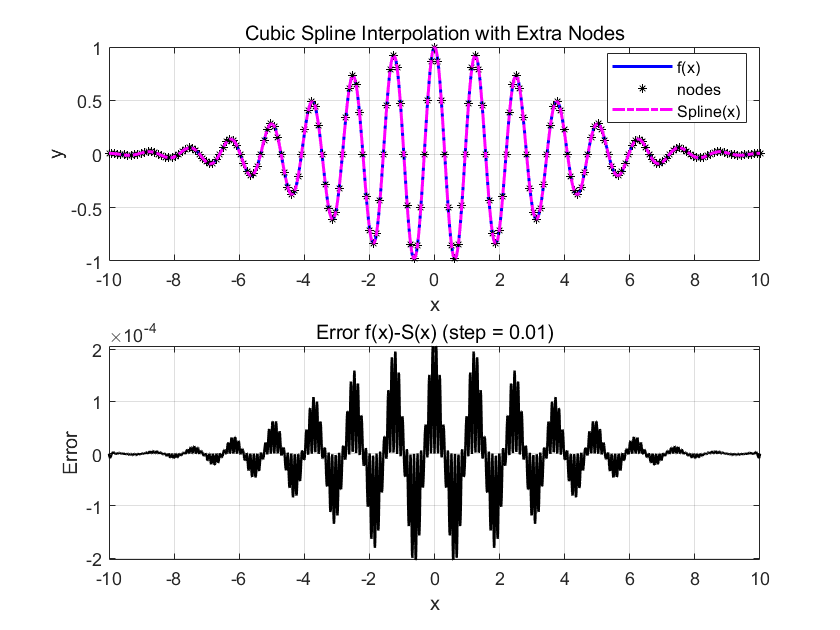
\includegraphics[width=\textwidth]{CS3.png}
    \caption{Cubic-Spline (2-more nodes)}
    \label{fig:nev_whole00}
  \end{subfigure}
  \hfill
  \begin{subfigure}[t]{0.48\textwidth}
    \centering
    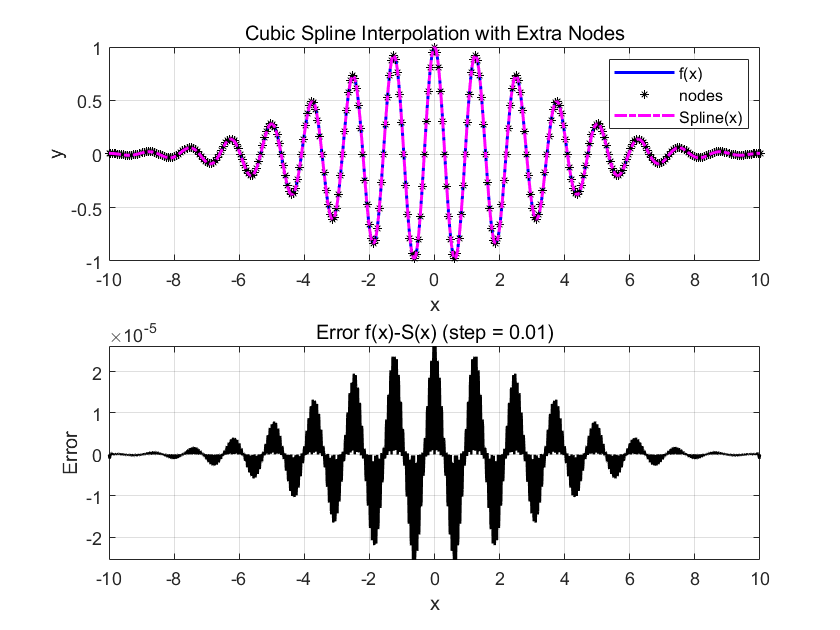
\includegraphics[width=\textwidth]{CS4.png}
    \caption{Cubic-Spline (4-more nodes)}
    \label{fig:nev_small00}
  \end{subfigure}
  \caption{Comparison of Cubic Spline added more nodes}
  \label{fig:nev_compare00}
\end{figure}
\FloatBarrier
It is not difficult to observe from these two generated images that the error of the CS method is not randomly distributed like VA method, 
but is positively correlated with the function value: the larger the function value, the greater the average error. Moreover, the error 
oscillates very rapidly. As mentioned earlier, the more nodes there are, the faster the oscillation becomes. With the increase in nodes, 
the error gradually decreases. However, its accuracy is significantly lower than that of the VA method, and the convergence speed of the 
error is approximately linear.\\
Thus, we have completed the discussion of two methods for reducing errors.

%Numerical Results
\section{Numerical Results} 

A summary of the performance and characteristics of each method is provided in Table3:
  \setlength{\tabcolsep}{8pt}  % 列间距
  \renewcommand{\arraystretch}{1.3}  % 行高
  \begin{table}[htbp]
    \centering
    \caption{Summary of Methods and Performance on $f(x)=e^{-x^2/20}\cos(5x)$ over $[-10,10]$}
    \label{tab:method_summary}
    \begin{tabular}{@{}p{0.16\textwidth} p{0.35\textwidth} p{0.35\textwidth}@{}}
      \toprule
      \textbf{Method} 
        & \textbf{Pros} 
        & \textbf{Cons} \\
      \midrule
      Taylor Series  
        & • Accurate near expansion point (local)  
        & • Poor global approximation; error grows exponentially\\
        & • Simple concept                        
        & • Very high order needed; formula complex     \\
      \addlinespace
      Neville's Method (equal nodes)  
        & • Conceptually simple; passes through all nodes  
        & • Severe Runge oscillations; large boundary error\\
      \addlinespace
      Cubic Spline  
        & • Piecewise smooth; avoids global oscillation  
        & • Slow (linear) error convergence;  \\
        & • Flexible node placement; No upper precision limit                 
        & • Accuracy lower than high-order VA     \\
      \addlinespace
      Vandermonde-Arnoldi with Chebyshev  
        & • Excellent global accuracy
        & • Algorithm is complex; Value at Chebyshev nodes needed\\
        & • Stable 
        & • Has precision limit around $10^{-14}$         \\
      \bottomrule
    \end{tabular}
  \end{table}
This section presents the key numerical results obtained from applying different approximation methods 
to $f(x) = e^{-x^2/20} \cos(5x)$ on $[-10, 10]$. The Taylor expansion demonstrates accuracy only in a very narrow region 
around $x=0$, with error increasing exponentially away from the origin (Figure 1&2). This highlights its fundamental limitation for 
approximating functions over large intervals.\\

Neville's method with equally spaced nodes (Figure 3) shows some local improvement over Taylor but suffers severely from the Runge 
phenomenon across the large interval. Extreme oscillations and large errors ($>10^6$) are observed near the boundaries, rendering it 
unsuitable for a global approximation of this function on $[-10, 10]$.

Cubic Spline interpolation (Figure 5, 6, 7), a piecewise polynomial method provides a smoother approximation compared to 
high-degree global polynomials and avoids the extreme Runge oscillations. Its error decreases with increasing node density and strategic 
node placement (including zeros and boundaries) improves its performance. However, the error magnitude correlates with the function's 
amplitude, and convergence is approximately linear, resulting in significantly lower accuracy ($\sim 10^{-2}$) compared to the best method 
tested.

The Vandermonde-Arnoldi (VA) method with Chebyshev nodes (Figure 4) proves to be the most effective 
technique for this problem. By utilizing Chebyshev nodes to mitigate boundary oscillations and employing a stable 
fitting algorithm, the VA method achieves remarkably high accuracy. At $n=100$, the error is reduced to the order of $10^{-15}$, 
demonstrating excellent global approximation and stability over the entire $[-10, 10]$ interval.



%Conclusions
\section{Conclusions}
This study systematically evaluates numerical methods for approximating the oscillatory Gaussian wave packet 
$f(x)=e^{-\frac{x^{2}}{20}}\ cos(5x)$ over [-10,10]. Taylor series expansions, while locally accurate near $x=0$
x=0, fail globally due to rapid error divergence beyond $|x|>5$. Neville's method with equidistant nodes exacerbates 
the Runge phenomenon, producing catastrophic oscillations $(>10^{6})$ near boundaries. Cubic spline interpolation offers 
piecewise smoothness but achieves only moderate accuracy $(~10^{-4})$ with linear error convergence tied to node density. 
In contrast, the Vandermonde-Arnoldi method with Chebyshev nodes emerges as the superior approach: at n=100, 
it attains machine-precision accuracy limit ($10^{-15}$) by mitigating Runge effects through optimal node distribution 
and orthogonal polynomial fitting. This method's stability and efficiency underscore its suitability for approximating 
high-frequency, decaying functions on extended domains. Future work could explore hybrid strategies integrating spline 
flexibility with global orthogonal bases for complex physical systems.


% Reference List(移除center环境)
\begin{thebibliography}{99}
\bibitem{bn} D. V.Shaykin, \textit{Analysis of modulated linear wave packets and gap solitons in coupled optical fibers}, arXiv 
preprint, 2024. Available: \url{https://arxiv.org/pdf/2504.21424}.

\bibitem{brubeck2021}
P. D. Brubeck, Y. Nakatsukasa and L. N. Trefethen, 
\textit{Vandermonde with Arnoldi},
SIAM Review, 63(2) (2021), pp.\ 405-415.

\bibitem{niu2023}
Q. Niu, H. Zhang and Y. Zhou,
\textit{Confluent Vandermonde with Arnoldi} 
Applied Mathematics Letters, 
vol.~135, 2023, art.~no.\ 108420.
\end{thebibliography}

\end{document}

